\section[Eigenzeugs]{Eigenwerte, Eigenvektoren und Eigenräume}
\Einleitung{Zunächst wagen uns noch einmal an Äquivalenzrelationen heran und schauen, wie wir damit Automorphismen eine Orientierung verleihen können.\\
Danach machen wir den ersten Schritt zur Diagonalisierung von Endomorphismen. Dies ist der Prozess, für einen Endomorphismus\footnote{der bestimmte Eigenschaften haben muss} $F\in \End(V)$ die Basis $B$ des zugrunde liegenden Vektorraums $V$ geschickt so zu wählen, dass die darstellende Matrix $M_B(F)$ nur noch Einträge auf der Diagonalen hat. Dazu müssen wir zunächst Begriffe wie Eigenwerte, Eigenvektoren und Eigenräume verstehen. Eigenvektoren sind Vektoren, die auf ein Vielfaches ihrer selbst\footnote{dieses Vielfache ist dann der Eigenwert} abgebildet werden, d. h. die Gleichung $A\Vec{v}=\lambda \Vec{v}$ erfüllen.\\
Ein wichtiges Werkzeug ist dabei das charakteristische Polynom, das wir auf endlichdimensionalen Vektorräumen verwenden können und das die Determinante zur Hilfe nimmt.}

\subsubsection{Basiswechsel und Orientierung von Automorphismen}
Die Mühe mit den Äquivalenzklassen haben wir uns vor allem gemacht, um gleich orientierte Basen als äquivalent einzustufen. Aber der Reihe nach:
\begin{Def}
{Basiswechsel}
Da die Basis von Vektorräumen nicht eindeutig ist, können wir lineare Abbildungen definieren, die von der einen in die andere Basis wechseln. Damit keine Information verloren geht, müssen diese bijektiv sein.\footnote{Wir betrachten also Automorphismen.}\\
Der \red{Basiswechsel} zwischen Basen $B$ und $B'$ von $V$ ist nun als folgende lineare Abbildung definiert:
\begin{equation}
    F:V\to V,\quad F(v)=\phi_{B'}(\phi_B^{-1}(v)),
\end{equation}
wobei $\phi_{B'}$ und $\phi_B$ lineare Abbildungen sind, für die die jeweiligen Basisvektoren spaltenweise in eine Matrix geschrieben werden.
\end{Def}
\begin{Beispiel}
{Basiswechsel im $\mathbb{R}^2$}
Wir betrachten $V=\mathbb{R}^2$ mit den Basen $B=\left\{\MatrixInline{1\\1},\MatrixInline{2\\0}\right\}$ und $B'=\left\{\MatrixInline{0\\2},\MatrixInline{1\\4}\right\}$.
Hier ist $\phi_B=\Matrix{1&2\\1&0}$ und $\phi_{B'}=\Matrix{0&1\\2&4}$.\footnote{denn z. B. gilt $\phi_B(\Vec{e}_1)=\Matrix{1\\1}\,\checkmark$}\\
Da wir von $B$ nach $B'$ wollen, müssen wir nun $\phi_B^{-1}$ bestimmen, also die inverse Matrix zu $\phi_B$ finden. Dafür nutzen wir die \href{https://de.wikipedia.org/wiki/Cramersche_Regel}{Cramersche Regel}:
\begin{equation*}
\phi_B^{-1}=\frac{1}{\det \phi_B}\Matrix{0&-2\\-1&1}\overset{\footnote{Es ist $\det \phi_B=-2$.}}{=}\frac{1}{2}\Matrix{0&2\\1&-1}.
\end{equation*}
Somit ist der Basiswechsel (bzw. dessen darst. Matrix) gegeben durch 
\begin{equation*}
F=\phi_{B'}\circ\phi_B^{-1}=\frac{1}{2}\Matrix{0&1\\2&4}\Matrix{0&2\\1&-1}=\Matrix{1&-1\\4&0}.
\end{equation*}
\end{Beispiel}



\begin{Def}
{Orientierung}
Wir nennen zwei Basen eines reellen Vektorraums \red{gleich orientiert}, wenn der Basiswechsel $F=\phi_{B'}\phi_B^{-1}: V\to V$ eine \underline{positive Determinante} hat.\\
\blue{Anmerkung: Da es sich um eine bijektive Abbildung handeln muss, ist $\det F$ niemals 0.}
\end{Def}

\begin{Beispiel}
{Orientierung des obigen Basiswechsels}
Für den Basiswechsel $B=\left\{\MatrixInline{1\\1},\MatrixInline{2\\0}\right\}\to B'=\left\{\MatrixInline{0\\2},\MatrixInline{1\\4}\right\}$ bedeutet das, dass die Basen gleich orientiert sind, denn $\det F= 1\cdot 0-(-1)4=4$.
\end{Beispiel}

\begin{Satz}{Folgerung}{Die Orientierung ist eine Äquivalenzrelation}
Wir können $B\sim B'\iff $ \textit{$B$ und $B'$ sind gleich orientiert} als Äquivalenzrelation auffassen.\\
Dann definiert jede Basis eine Äquivalenzklasse $[B]$ bzw. eine Orientierung. Es gibt genau zwei Orientierungen.
\end{Satz}

\begin{Def}
{Positive Orientierung}
Wir nennen $B$\footnote{Basis von $V$ mit $\dim V=n$.} \red{positiv orientiert}, wenn sie dieselbe Orientierung wie die kanonische Basis $B_e=\{\Vec{e}_1,\ldots,\Vec{e}_n\}$ hat. Andernfalls nennen wir $B$ \red{negativ orientiert}.
\end{Def}
Dieses Konzept kennt ihr bestimmt schon aus dem $\mathbb{R}^3$: Die kanonische Basis und alle positiv orientierten Basen könnt ihr mit der \textit{Rechte-Hand-Regel} nachvollziehen, alle anderen mit der linken Hand.
\begin{Beispiel}{Orientierung zweier Basen}
\begin{wrapfigure}{r}[0pt]{.35\textwidth}
 \vspace{-15pt}
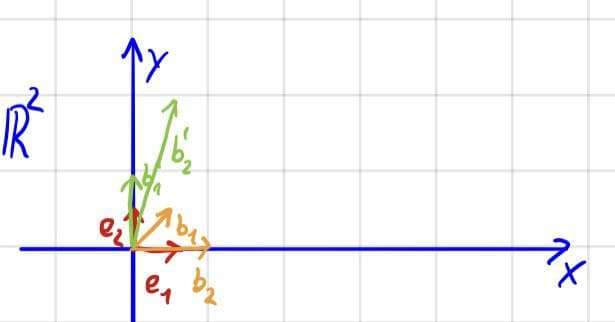
\includegraphics[width=.35\textwidth]{Dateien/01/01Basiswechsel.jpg}
 \vspace{-15pt}
\end{wrapfigure}
Der Basiswechsel von $B_e\to B$ ist sehr einfach, da $\phi_{B_e}^{-1}=\phi_{B_e}=\mathds{1}_n$. Also müsst ihr für den Basiswechsel von $B_e\to B$  eigentlich nur die Determinante von $\phi_B$ berechnen.\\
Wir betrachten wieder $B=\left\{\MatrixInline{1\\1},\MatrixInline{2\\0}\right\}$.\\
Hier ist $\det(\phi_B\circ\phi_{B_e}^{-1})=\det\phi_B=\det\MatrixInline{1&2\\1&0}=-2$.\\
Somit ist $B$ nicht gleich wie die kanonische Basis, also negativ orientiert.\\
Aufgrund der vorigen Feststellung, weil $B\sim B'$, ist auch $B'$ negativ orientiert. Alternativ ergibt das auch der folgende Test:\\ $\det(\phi_{B'}\circ\phi_{B_e}^{-1})=-2$.
\end{Beispiel}

\begin{Def}{Orientierung eines Automorphismus}
Abgesehen von Basiswechseln nennen wir allgemein Automorphismen $F\in \GL(V)$ \red{orientierungserhaltend}, wenn $\det F>0$.\\
Analog nennen wir $F$ \red{orientierungsumkehrend}, wenn $\det F<0$.
\end{Def}

%%%%%%%%%%%%%%%%%%%%%%%%%%%%%%%%%%%%%%
\subsection{Mathematische Eigenartigkeiten - Eigenwerte und Eigenvektoren}
\begin{Def}
{Eigenwert und Eigenvektor}
Wird ein Vektor $\Vec{v}$\footnote{der nicht der Nullvektor ist!} durch einen Endomorphismus $F\in\End(V)$ auf ein Vielfaches $\lambda$ seiner selbst abgebildet, so nennen wir ihn \red{Eigenvektor} von $F$. Der Skalierungsfaktor $\lambda$ ist der zugehörige \red{Eigenwert}.\\
Anders geschrieben: $\Vec{v}$ erfüllt die \underline{Eigenwertgleichung}
\begin{equation}
\boxed{F(\Vec{v})=\lambda \Vec{v}}, \quad \Vec{0}\neq \Vec{v}\in V,\quad \lambda \in \mathbb{K}.
\end{equation}
\blue{Zu einem Eigenwert kann es verschiedene Eigenvektoren geben!}
\end{Def}

\begin{Def}
{Eigenraum}
Das lineare Erzeugnis aus allen Eigenvektoren zu einem gegebenen Eigenwert $\lambda$ nennen wir \red{Eigenraum} zum Eigenwert $\lambda$. Dieser ist stets ein Unterraum von $V$, wir schreiben
\begin{equation}
V_\lambda=\Menge{\Vec{v}\in V}{F(\Vec{v})=\lambda \Vec{v}}=\Span{\Vec{v}\in V}{\Vec{v} \tx{ ist Eigenvektor zu } \lambda}.
\end{equation}
\end{Def}

Wir schauen uns gleich die geometrische Bedeutung dieser Definitionen an, doch vorher ein paar Beispiele und Rechenregeln:
\begin{Beispiel}{Eigenzeugs im $\mathbb{R}^2$}
Betrachte $V=\mathbb{R}^2,\, F:=\MatrixInline{0&1\\1&0}\in \End(V)$.\\
Die Eigenwertgleichung ergibt dann:
\begin{equation*}
F(\Vec{v})=\lambda \Vec{v}\iff \Matrix{0&1\\1&0}\Matrix{x\\y}=\Matrix{\lambda x\\\lambda y}\iff y =\lambda x,\, x=\lambda y\implies y=\lambda^2 y\implies \lambda=\pm 1.
\end{equation*}
Die Eigenwerte sind also $\lambda=\pm 1$.\\
Für $\lambda_1=+1$ gilt $y=x$, also ist z. B. $\Vec{v}=\MatrixInline{1\\1}$ ein Eigenvektor zu $\lambda_1$.\\
Für $\lambda_2=-1$ gilt $y=-x$, also ist z. B. $\Vec{v}=\MatrixInline{-1\\1}$ ein Eigenvektor zu $\lambda_2$.\\
Die Eigenräume sind dann $V_{\lambda_1}=\Spann{\MatrixInline{1\\1}}$ und $V_{\lambda_2}=\Spann{\MatrixInline{-1\\1}}$\\
Es gibt nicht mehr Eigenwerte, da die Summe der Dimensionen der Eigenräume (hier $1+1=2$) stets kleiner gleich $\dim V$ ist (dazu später mehr).
\end{Beispiel}

\subsubsection{Das charakteristische Polynom}
\blue{\textbf{Motivation}:\\
Wir lernen nun ein wichtiges Werkzeug zur Bestimmung von Eigenwerten auf \textbf{endlich\-dim\-ension\-al\-en} Vektorräumen kennen:\\
\textbf{Das charakteristische Polynom}.\\
Wie sieht es aus? Und woher kommt das? Wir betrachten eine kurze Herleitung und gehen dafür von der bekannten Eigenwertgleichung aus:
\begin{alignat*}{2}
A\Vec{v}&=\lambda \Vec{v}&\furdas\tx{Wir formen nun einfach um: Es ist $\Vec{w}=\mathds{1}_n \Vec{w}\quad\forall \Vec{w}\in V$.}\\
\iff A\Vec{v} &=\mathds{1}_n(\lambda \Vec{v})&\furdas-\mathds{1}_n(\lambda \Vec{v}) \tx{ und Assoziativität: }\mathds{1}_n(\lambda \Vec{v})=(\mathds{1}_n\lambda)\Vec{v}.\\
\iff A\Vec{v}-\mathds{1}_n\lambda \Vec{v}&=\Vec{0}&\furdas \tx{Klammere $\Vec{v}$ aus. Zudem ist $\mathds{1}_n\lambda=\lambda\mathds{1}_n$, weil $\lambda$ ein Skalar ist.}\\
\iff (A-\lambda\mathds{1}_n)\Vec{v}&=\Vec{0}&\furdas\tx{Diese Gleichung kann nur erfüllt sein, wenn $\det(A-\lambda\mathds{1}_n)=0$ ist.}\\
\implies \det(A-\lambda\mathds{1}_n)&=0&\furdas \tx{Dies ist nun unser Werkzeug zum Finden von Eigenwerten.}
\end{alignat*}}
\begin{Def}{Charakteristisches Polynom}
Für $V$ mit $\dim V=n<\infty$ definieren wir für Endomorphismen $F\in \End(V)$ das \red{charakteristische Polynom} $P_F(\lambda)$ mit
\begin{equation}
P_F:\mathbb{K}\to\mathbb{K},\quad\boxed{P_F(\lambda)=\det(F-\lambda\Id)=\det(A-\lambda\mathds{1}_n)}
\end{equation}
wobei $A$ die darstellende Matrix von $F$ bzgl. einer beliebigen Basis von $V$ sei.
\end{Def}
\begin{Satz}{Satz}{Eigenwerte sind Nullstellen des charakteristischen Polynoms}
Die Eigenwerte von $F$ sind genau die Nullstellen des charakteristischen Polynoms, d. h.
\begin{equation}
\boxed{\det(A-\lambda\mathds{1}_n)=0}\impliedby \lambda\tx{ ist Eigenwert von }F.
\end{equation}
\end{Satz}
\begin{Beispiel}{Bestimmung von Eigenwerten}
Betrachte $F:V\to V$ mit der darst. Matrix $A=\MatrixInline{2&1\\3&0}$ bzgl. der kanonischen Basis. Diese hat die Eigenwerte $\lambda_1=-1$ und $\lambda_2=3$, denn
\begin{align*}
P_F(\lambda)&=\det(A-\lambda\mathds{1}_2)=\det\Matrix{2-\lambda&1\\3&-\lambda}=-2\lambda+\lambda^2-3\overset{!}{=}0\\
\overset{p-q}{\iff}\lambda_{1,2}&=-\frac{-2}{2}\pm\sqrt{1-(-3)}=1\pm 2.
\end{align*}
Nun können wir auch die Eigenvektoren bestimmen.\\
Dafür müssen wir das Gleichungssystem $A\Vec{v}=\lambda_i\Vec{v}$ lösen.\\
\begin{eqnarray*}
\lambda_1:\quad \Matrix{2&1\\3&0}\Matrix{x\\y}&=&-1\Matrix{x\\y}\overset{\footnote{Diesen Schritt würde ich immer empfehlen}}{\iff} \Matrix{3&1\\3&1}\Matrix{x\\y}=\Matrix{0\\0}\\
\overset{\footnote{Gauß-Schreibweise}}{\iff}\MatrixInvertieren{3&1\\3&1}{0\\0}&\overset{\tx{II}-\tx{I}}{\longrightarrow}&\MatrixInvertieren{3&1\\0&0}{0\\0}\implies y=t\in\mathbb{R}\tx{ bel.}\\
\iff 3x&=&-y\iff x=-\frac{t}{3}\\
\tx{Wähle $t=3$: }\implies \Vec{v}&=&\Matrix{-1\\3} \tx{ ist Eigenvektor.}\\
\tx{Der Eigenraum ist dann } V_{\lambda_1}&=&\Spann{\Matrix{-1\\3}}.\\
\lambda_2:\quad \Matrix{2&1\\3&0}\Matrix{x\\y}&=&3\Matrix{x\\y}\\
\overset{\footnote{Gauß-Schreibweise}}{\iff}\MatrixInvertieren{-1&1\\3&-3}{0\\0}&\overset{\tx{II}+3\tx{I}}{\longrightarrow}&\MatrixInvertieren{-1&1\\0&0}{0\\0}\implies y=t\in\mathbb{R}\tx{ bel.}\\
\iff -x&=&-y\iff x=t\\
\tx{Wähle $t=1$: }\implies \Vec{v}&=&\Matrix{1\\1} \tx{ ist Eigenvektor.}\\
\tx{Der Eigenraum ist dann } V_{\lambda_2}&=&\Spann{\Matrix{1\\1}}
\end{eqnarray*}
\end{Beispiel}

\begin{Def}
{Multiplizität der Nullstellen}
Ganz allgemein können wir jedes Polynom auch als Produkt seiner Nullstellen\footnote{bzw. $(x-x_0)$ etc.} und einem nicht-Null werdenden Rest schreiben.\\
Betrachten wir nur eine bestimmte Nullstelle, so können wir diese aus dem Rest \textit{herausziehen}:
\begin{equation*}
P(\lambda)=(\lambda-\lambda_i)^m\cdot Q(\lambda),
\end{equation*}
wobei $\lambda_i$ die Nullstelle und $Q(\lambda)$ der Rest (ebenfalls ein Polynom), für den $Q(\lambda_i)\neq 0$ gilt, sind.\\
Wir nennen die Potenz $m$ die \red{Vielfachheit} der Nullstelle $\lambda_i$.
\end{Def}

\begin{Beispiel}{Vielfachheit eines Polynoms}
Wir betrachten als Beispiel
\begin{equation*}
P(\lambda)=(\lambda-5)^3(\lambda+2)27(\lambda^2+1)
\end{equation*}
Hier hat $\lambda_1=5$ die Vielfachheit 3 und $\lambda_2=-2$ die Vielfachheit 1. Es gibt keine weitere Nullstelle.
\end{Beispiel}

\begin{Def}
{Algebraische Vielfachheit}
Im Zusammenhang mit dem charakteristischen Polynom von $F\in\End(V)$ nennen wir die Vielfachheit der Nullstelle $\lambda_i$ des char. Polynoms, die ja mit dem Eigenwert $\lambda_i$ korrespondiert, die \red{algebraische Vielfachheit $m_{\lambda_i}$} von $\lambda_i$.
\end{Def}

\begin{Def}
{Geometrische Vielfachheit}
Dem gegenüber steht die \red{geometrische Vielfachheit $n_{\lambda_i}$} des Eigenwertes $\lambda_i$, welche als Dimension des zu $\lambda_i$ gehörigen Eigenraumes\footnote{also die Anzahl der zum Eigenwert gehörigen linear unabhängigen Eigenvektoren.} definiert ist, d. h. $n_{\lambda_i}=\dim V_{\lambda_i}$.
\end{Def}

\begin{Satz}{Satz}{Beschränkung der Vielfachheiten}
Während die Summe aller algebraischen Vielfachheiten durch $\dim V=\grad P_F(\lambda)=n$ beschränkt ist, ist für jeden Eigenwert $\lambda_i$ die geometrische durch die algebraische Vielfachheit beschränkt, d. h.
\begin{equation}
\boxed{n_{\lambda_i}\leq m_{\lambda_i}}\quad \tx{und }\sum_{i=1}^km_{\lambda_i}\leq n=\dim V\tx{ mit $k$ der Anzahl der Eigenwerte.}
\end{equation}
\end{Satz}

\begin{Satz}{Satz}{Eigenvektoren sind linear unabhängig}
Die Familie der Eigenvektoren $(\Vec{v}_i)_{i=1...k}$ zu paarweise verschiedenen Eigenwerten ist linear unabhängig.\\
Wir sehen also:\\
Wenn die Summe der geometrischen Vielfachheiten $\sum_{i=1}^k n_{\lambda_i}=n=\dim V$ ist, gibt es also $n$ linear unabhängige Eigenvektoren. Diese bilden wiederum eine Basis von $V$, es ist $V=V_{\lambda_1}\oplus V_{\lambda_2}\oplus\ldots\oplus V_{\lambda_k}$, der Vektorraum wird in diesem Fall also durch die Eigenvektoren aufgespannt und ist die direkte Summe der Eigenräume!\\
Wir werden sehen, dass diese Basis spezielle Eigenschaften hat.
\end{Satz}

\begin{Beispiel}{Eigenwerte und Eigenräume}
Wir berechnen die Eigenwerte und Eigenräume zum Endomorphismus
\begin{equation*}
F: V\to V,\quad A_F=\Matrix{3&4&-3\\2&7&-4\\3&9&-5}.
\end{equation*}
Das charakteristische Polynom ist mit der Regel von Sarrus \eqref{eq:Sarrusregel}
\begin{align*}
P_F(\lambda)&=\det(A-\lambda\mathds{1}_n)\\
&=(3-\lambda)(7-\lambda)(-5-\lambda)+3(-4)4+2\cdot 9(-3)-2\cdot 4(-5-\lambda)\\
&\quad-(3-\lambda)9(-4)-3(-3)(7-\lambda)\\
&=-\lambda^3+5\lambda^2-8\lambda+4\overset{!}{=}0.
\end{align*}
Wir erraten die erste Nullstelle, $\lambda_1=1$.\\
Eine Polynomdivision ergibt $P_F(\lambda)/(\lambda-1)=-(\lambda-2)^2$.\\
Also ist $\lambda_2=2$ und wir können schreiben
\begin{equation*}
P_F(\lambda)=-(\lambda-1)^1(\lambda-2)^2\implies m_{\lambda_1}=1,\,m_{\lambda_2}=2.
\end{equation*}
\begin{wrapfigure}{r}[0pt]{.35\textwidth}
 \vspace{-15pt}
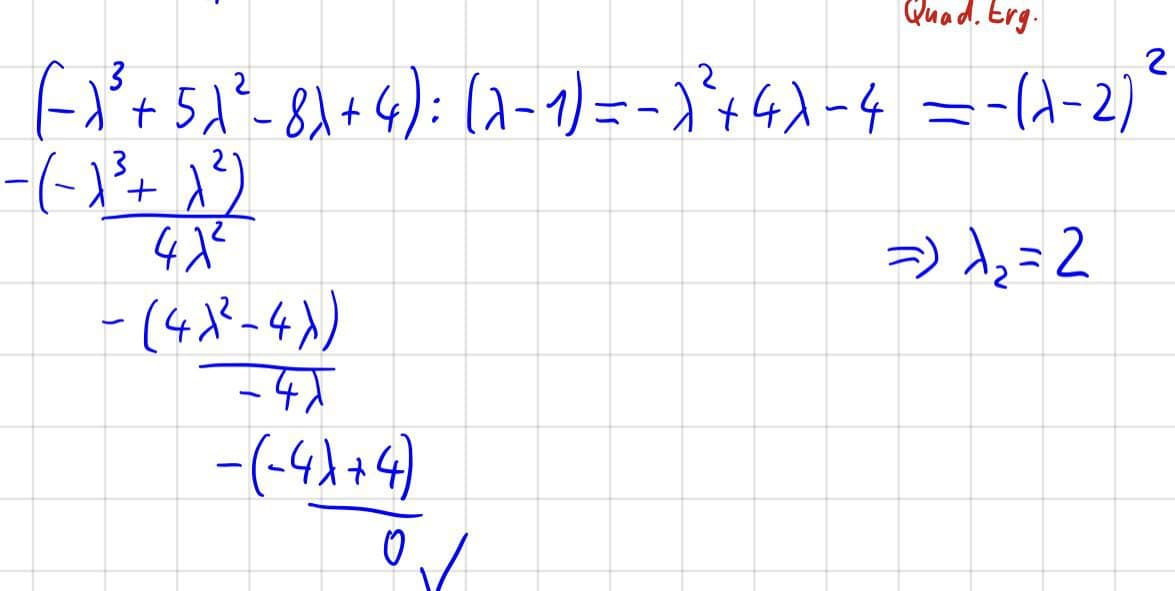
\includegraphics[width=.35\textwidth]{Dateien/01/01PolDiv.jpg}
 \vspace{-15pt}
\end{wrapfigure}
Wir bestimmen die Eigenvektoren und ziehen dafür direkt $\lambda_i$ auf der Hauptdiagonalen ab:
\begin{align*}
\lambda_1:\quad &\MatrixInvertieren{2&4&-3\\2&6&-4\\3&9&-6}{0\\0\\0}\overset{\frac{2}{3}\tx{III}}{\longrightarrow}\MatrixInvertieren{2&4&-3\\2&6&-4\\2&6&-4}{0\\0\\0}\\
&\overset{\tx{III}-\tx{II},\,\tx{II}-\tx{I}}{\longrightarrow}\MatrixInvertieren{2&4&-3\\0&2&-1\\0&0&0}{0\\0\\0}\implies z=t\in\mathbb{R}\tx{ bel.}\\
&\implies 2y=z\iff y=\frac{t}{2}\implies 2x=3z-4y\iff x=\frac{3}{2}t-t\\
&\overset{\tx{Wähle }t=2}{\implies} \Vec{v}=\Matrix{1\\1\\2}\longrightarrow V_1=\Spann{\Matrix{1\\1\\2}}\\
\lambda_2:\quad &\MatrixInvertieren{1&4&-3\\2&5&-4\\3&9&-7}{0\\0\\0}\overset{6\tx{I},\,3\tx{II},\,2\tx{III}}{\longrightarrow}\MatrixInvertieren{6&24&-18\\6&15&-12\\6&18&-14}{0\\0\\0}\overset{\II-\I,\,\III-\I}{\longrightarrow}\MatrixInvertieren{6&24&-18\\0&-9&6\\0&-6&4}{0\\0\\0}\\
&\overset{2\II,\,3\III}{\longrightarrow}\MatrixInvertieren{6&24&-18\\0&-18&12\\0&-18&12}{0\\0\\0}\overset{\I/6,\,\III-\II,\, \II/6}{\longrightarrow}\MatrixInvertieren{1&4&-3\\0&-3&2\\0&0&0}{0\\0\\0}.
\end{align*}
Schon hier sehen wir, dass $\dim V_2=1$ ist, da wir nur eine Nullzeile haben. Somit ist $n_{\lambda_1}=1<2=m_{\lambda_2}$.
\begin{align*}
&\implies z=t\in\mathbb{R}\tx{ bel.} \implies 3y=2z\iff y=\frac{2}{3}t\implies x=3z-4y=3t-\frac{8}{3}t.\\
&\overset{\tx{Wähle }t=3}{\implies}\Vec{v}=\Matrix{1\\2\\3}\to V_{\lambda_2}=\Spann{\Matrix{1\\2\\3}}.
\end{align*}
Wir sehen also: Die Eigenvektoren sind zwar linear unabhängig, können aber keine Basis des $\mathbb{R}^3$ bilden, da es zu wenige sind.
\end{Beispiel}


\subsubsection{Exkurs: Geometrische Bedeutung von Eigenvektoren}
Betrachten wir den $\mathbb{R}^2$ oder $\mathbb{R}^3$, so \red{drehen, strecken oder stauchen} Endomorphismen\footnote{Ein letztes Mal: Lineare Abbildungen eines Vektorraums in sich selbst.} Vektoren.\\
Eigenvektoren sind nun genau jene Vektoren, die durch die Abbildung \underline{nicht} gedreht, sondern \textit{nur} skaliert werden. Der Skalierungsfaktor ist genau der Eigenwert $\lambda$.

\begin{Beispiel}{Drehmatrix (1/2)}
Die Drehmatrix $D_\varphi:\mathbb{R}^2\to\mathbb{R}^2,\quad \Vec{v}\mapsto D_\varphi \Vec{v},\quad D_\varphi=\MatrixInline{\cos\varphi&-\sin\varphi\\\sin\varphi&\cos\varphi}$ mit\\
$D_\varphi\MatrixInline{x\\y}=\MatrixInline{x\cos\varphi-y\sin\varphi\\x\sin\varphi+y\cos\varphi}$ ($\varphi\in[0,2\pi)$) ist ein Endomorphismus.\footnote{und sogar ein Isomorphismus, da $\det D_\varphi=\cos^2\varphi+\sin^2\varphi=1\,\forall\varphi$}\\
Berechnen wir die Eigenwerte:\\
Was erwarten wir? Im Reellen sollten wir nur für $\varphi=0$ und $\varphi=\pi\hat{=}180^\circ$ nicht gedrehte (und sogar nicht skalierte, bis auf den Faktor $-1$) Vektoren finden.\\
Wir betrachten das charakteristische Polynom:
\begin{align*}
P_{D_\varphi}(\lambda)&=\det(D_\varphi-\lambda\mathds{1}_2)=\det\Matrix{\cos\varphi-\lambda&-\sin\varphi\\\sin\varphi&\cos\varphi-\lambda}\\
&=\cos^2\varphi-2\cos\varphi\lambda+\lambda^2+\sin^2\varphi=\lambda^2-2\cos\varphi\lambda+1\overset{!}{=}0\\
\implies \lambda_{1,2}&=\cos\varphi\pm\sqrt{\cos^2\varphi-1}=\cos\varphi\pm\sqrt{-\sin^2\varphi}.
\end{align*}
Wir sehen also direkt, dass reelle Eigenwerte nur für $\varphi\in\Menge{a\in\mathbb{R}}{a=n\pi,\,n\in\mathbb{Z}}$ möglich sind, wenn $\sin\varphi=0$ ist.\\
Im betrachteten Intervall ist das genau $\varphi=0$ ($\lambda=1$) und $\varphi=\pi$ ($\lambda=-1$). Es gibt dann also nur einen Eigenwert.\\
Wir betrachten den Fall $\varphi=\pi$. In diesem Fall ist $D_\pi=\MatrixInline{-1&0\\0&-1}$.\\
Eine Lösung des Gleichungssystems für $\lambda=-1$ ergibt
\begin{equation*}
    \MatrixInvertieren{-1-(-1)&0\\0&-1-(-1)}{0\\0}=\MatrixInvertieren{0&0\\0&0}{0\\0}\implies \Vec{v}=\Matrix{r\\t},\,r,t\in\mathbb{R}.
\end{equation*}
Der Eigenraum zu $\lambda_1=-1$ ist also $V_1=\Spann{\MatrixInline{1\\0},\MatrixInline{0\\1}}$. Dies ergibt auch geometrisch Sinn, denn die Matrix spiegelt ja jeden Vektor nur.\\
Hier haben wir also ein Beispiel, wo $n_\lambda=m_\lambda=2$ ist.
\end{Beispiel}

\begin{Beispiel}
{Abbildende Matrix im $\mathbb{R}^2$ (2/2)}
\begin{wrapfigure}{r}[0pt]{.15\textwidth}
 \vspace{-15pt}
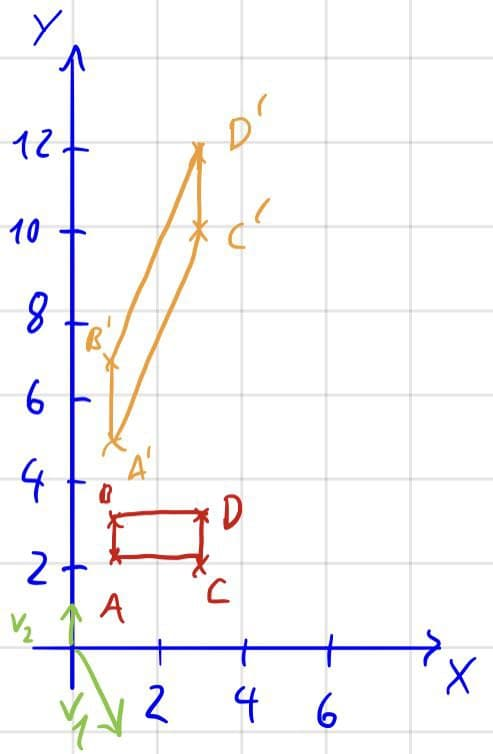
\includegraphics[width=.15\textwidth]{Dateien/02/02Anschauung1.jpg}
 \vspace{-15pt}
\end{wrapfigure}
Gegeben sei $F:\mathbb{R}^2\to\mathbb{R}^2,\,\Vec{v}\mapsto A_F\Vec{v}$ mit der darstellenden Matrix\\
$A_F=\MatrixInline{1&0\\2&2}$.\\
Sei nun $R$ ein Rechteck mit den Eckpunkten\\
$A=\MatrixInline{1\\2},\,B=\MatrixInline{1\\3},\,C=\MatrixInline{3\\2},\,D=\MatrixInline{3\\3}$.\\
Das Bild des Rechtecks können wir dann auch ermitteln.
Wir kennzeichnen die Eckpunkte des Bildes mit einem $'$:
\begin{equation*}
    A_F(A):=A'=\Matrix{1&0\\2&2}\Matrix{1\\2}=\Matrix{1\\6},\,B'=\Matrix{1\\8},\,C'=\Matrix{3\\10},\,D'=\Matrix{3\\12}.
\end{equation*}
Wir berechnen die Eigenwerte von $A$ mithilfe des charakteristischen Polynoms\\ $P_F(\lambda)=(1-\lambda)(2-\lambda)$ und lesen ab, dass $\lambda_1=1$ und $\lambda_2=2$.\\
Wir suchen die Eigenvektoren mithilfe der Eigenwertgleichung $A\Vec{v}=\lambda \Vec{v}\iff (A-\lambda\mathds{1}_2)\Vec{v}=\Vec{0}$ und verwenden dafür die Gaußschreibweise:
\begin{align*}
    \lambda_1:&\,\MatrixInvertieren{0&0\\2&1}{0\\0}\to x=t, \,y=-2t\implies \Vec{v}_1=t\Matrix{1\\-2}\to \tx{ER: } \Spann{\Matrix{1\\-2}}\\
    \lambda_2:&\, \MatrixInvertieren{-1&0\\2&0}{0\\0}\overset{\II+2\I}{\longrightarrow}\MatrixInvertieren{-1&0\\0&0}{0\\0}\to y=t,\,x=0\implies \Vec{v}_2=t\Matrix{0\\1}\to\tx{ER: }\Spann{\Matrix{0\\1}}.
\end{align*}
Wir sehen in der Skizze, dass jegliche Verbindungen in y-Richtung um den Faktor 2 gestreckt werden. Dies ist quasi genau der zweite Eigenwert/Eigenvektor.\\
Im Übrigen stellt die Matrix also eine Scherung im $\mathbb{R}^2$ dar, die, weil $\det A_F=2$, den Flächeninhalt geometrischer Figuren verdoppelt und dabei die Orientierung erhält.\\
Die Fixpunkte sind die Eigenvektoren, d. h. eine Figur mit Kanten, die diesen entsprechen, würde nicht geschert werden.\\
Betrachten wir folgendes Parallelogramm, das die Eigenvektoren von $A_F$ als Kanten hat:
\begin{align*}
    P_A&=\Matrix{0\\0},\,P_B=\Matrix{0\\2},\,P_C=\Matrix{1\\0},\,P_D=\Matrix{1\\-2}\\
    \to A(P_A):=P_A'&=\Matrix{1&0\\2&2}\Matrix{0\\0}=\Matrix{0\\0},\,P_B'=\Matrix{0\\4},\,P_C'=\Matrix{1\\2},\,P_D'=\Matrix{1\\-2}.
\end{align*}
\begin{center}
    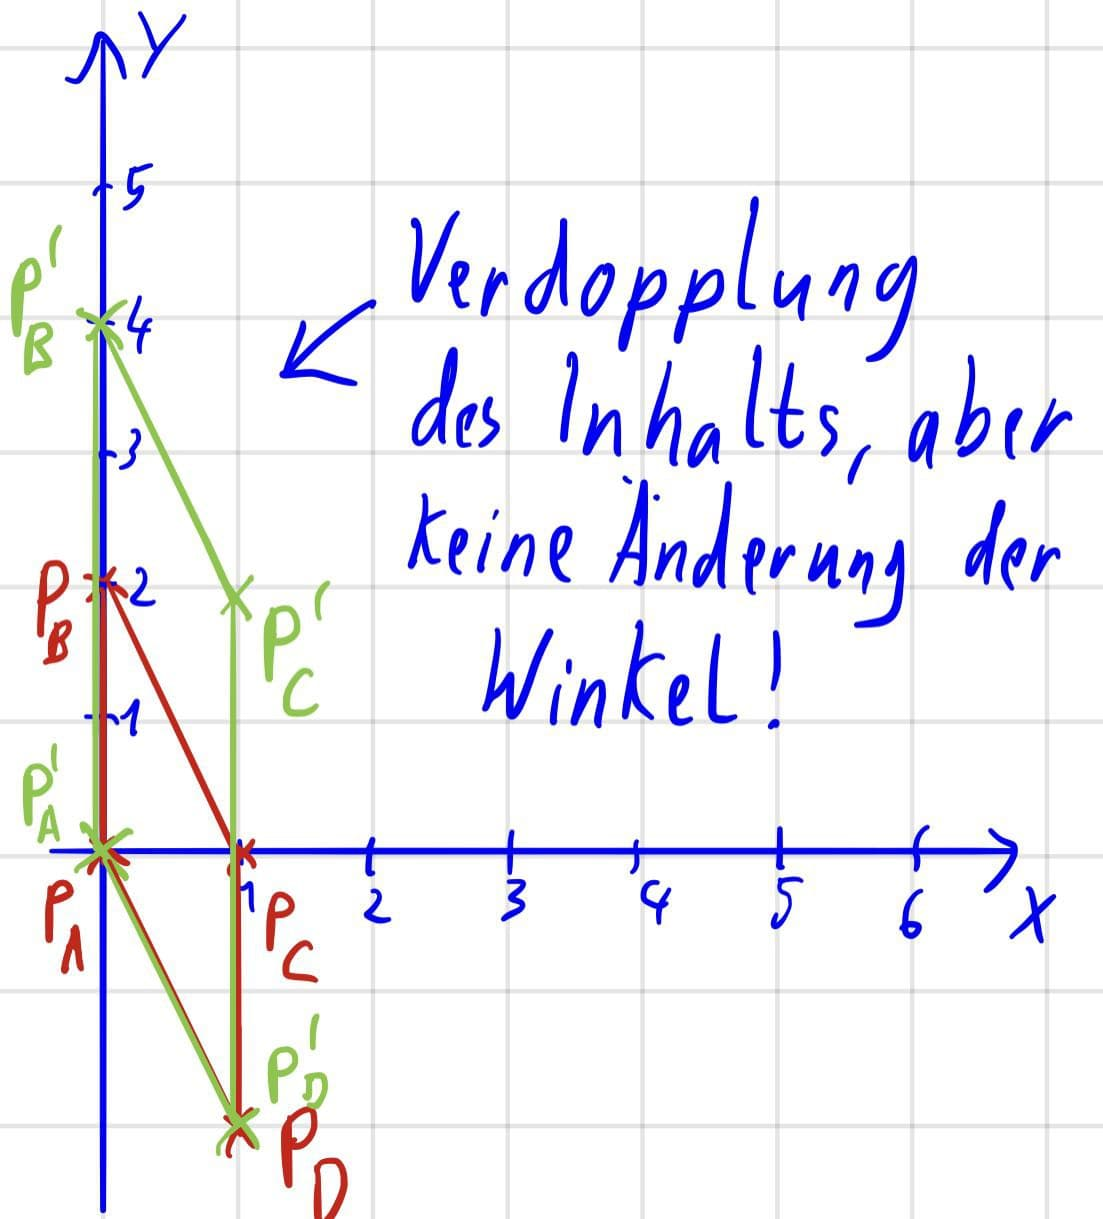
\includegraphics[width=.25\textwidth]{Dateien/02/02Anschauung2.jpg}
\end{center}
Es wird durch also tatsächlich nur geschert.
\end{Beispiel}


\Tipps{2}{
\begin{enumerate}
    % \item Orientiert euch an unseren Beispielen und überprüft genau, ob alle Axiome für eine Äquivalenzrelation erfüllt sind. Bei a) ist mit der Standard-Abstandsfunktion einfach $d(x,y)=\Abs{x-y}$ gemeint.\\
    % Beachtet bei b), dass nur alle durch drei teilbaren ganzen Zahlen gemeint sind (damit es nicht schon an der Reflexivität scheitert - sonst wäre nämlich z. B. $x=2$ nicht zu sich selbst äquivalent, da $2+2=4$ nicht durch 6 teilbar ist. Bei der Transitivität lohnt sich bei b) ein Blick auf den Beweis der Reflexivität.\footnote{Falls diese Aussage stimmen solte ;)}
    \item Das Invertieren der Matrix sollte mit unseren Beispielen von letzter Woche kein Problem sein. Mithilfe der Determinanten könnt ihr (zumindest notwendig) überprüfen, ob ihr richtig liegt.\footnote{Wenn ihr ganz sichergehen wollt, könnt ihr natürlich auch $A^{-1}A$ berechnen.}
    \item Hierzu b) gibt Robin in unserem Tutorium noch ein paar Tipps. 
    \item Dies ist ein Einzeiler. Startet mit der Definition des Betrages und macht euch dann klar, wie eine Matrix mit $(\overline{u_{ji}})$ aussieht.
    % \item \begin{enumerate}
    %     \item Hier hilft es, die Linearität der Determinante auszunutzen - welche Spalte bietet sich dafür an? Denkt dann an den Gauß-Algorithmus.\\
    %     Ihr solltet bei einem Ausdruck der Form
    %     \begin{equation*}
    %         \det A= \prod_{i=1}^n a_i+\sum_{k=1}^nb_k\prod_{j\neq k}^n c_j
    %     \end{equation*}
    %     kommen.
    %     \item Wir sehen leider nicht, wie man das mit Induktion macht, wir haben das mithilfe eines direkten Beweises und Aufgabe 3a) gemacht. Auch hier gilt wieder: Linearität ausnutzen!\\
    %     Weiterer Tipp (der in ähnlicher Form vielleicht nützlich ist):
    %     \begin{equation*}
    %         \det\Matrix{a_1&a_2&a_3\\a_1&a_2&a_3\\a_1&a_2&a_3}=\prod_{i=1}^3a_i\det\Matrix{1&1&1\\1&1&1\\1&1&1}
    %     \end{equation*}
    % \end{enumerate}
    \item Geht ganz klassisch nach dem Induktionsprinzip vor. Für den Induktionsanfang schaut euch noch einmal an, wie das leere Produkt definiert ist.\\
    Der Rest der Induktion ist ziemlich kompliziert, ihr könnt z. B. folgendermaßen vorgehen: Für $n+1$ wollt ihr ja irgendwie darauf hinaus, die Induktionsvoraussetzung einzusetzen. Dafür müsst ihr unter anderem die Linearität (bzw. Gauß'sche Umformungen) ausnutzen, um eine entspannte Laplace-Entwicklung machen zu können.\\
    Die entwickelte Matrix müsst ihr vermutlich ein bisschen länger angucken, Stichwort \textit{Determinantenmultiplikationssatz}.\\
    Wir hoffen, dass das hilft, lasst euch nicht von dem kompliziert aussehenden Produkt entmutigen, ihr schafft das! :)
    \item Hier ganz stumpf wie vorgeschlagen den Laplaceschen Entwicklungssatz auf $P_A(\lambda)=\det(A-\lambda\mathds{1}_n)$ anwenden.\\
    Heraus kommen sollte eine Summe der Form $\sum_{k=0}^{n-1}a_k$ (bzw. $\sum_{k=1}^nb_k$ wenn ihr den Index anders wählt).\\
    Anschließend müsst ihr mit vollst. Induktion zeigen, dass dies richtig ist. Auch hier hilft Laplace!
\end{enumerate}
}